\section{Fixed Expansion to Four Additional Tasks}
\label{app:new-task-expansion}
This exploratory expansion fixes four tasks before its formal runs:
CiteSeer/GCN \citep{kipf2017gcn} with a rank-4 input adapter; a synthetic sphere signed
distance field with a rank-8 SIREN \citep{sitzmann2020siren}; Burgers solution-operator learning
with a rank-8 DeepONet \citep{lu2019deeponet}; and $128\times128$ rank-8 matrix completion
with planted condition number 100. It is an additional task study,
not an independently confirmed or completed exhaustive proposal grid.
The SDF is synthetic. Burgers uses the documented Cole--Hopf
quadrature data and parameter-held-out splits from
Appendix~\ref{app:full-protocol}; it is not relabeled as a public
benchmark data set.

Each task crosses all four methods with exactly the same nine learning
rates
\[
\{10^{-5},3\!\times\!10^{-5},10^{-4},3\!\times\!10^{-4},
10^{-3},3\!\times\!10^{-3},10^{-2},3\!\times\!10^{-2},10^{-1}\}.
\]
We fix $\beta=0.9$, $\varepsilon=10^{-6}$, balance interval one,
and seed 42. The two larger step sizes extend the proposal's original
learning-rate slice equally for every method, to examine the
underfitting seen at its central setting. Graph runs have 1000 epochs;
the other runs have 2000. The four task blocks contain 36 attempts
each, for 144 total. Low-resource execution checks provide timing
estimates only and never enter the result tables.

\paragraph{Validation and test separation.}
Within a run, the earliest minimum-validation-loss checkpoint is
selected: cross-entropy for graphs and MSE for the other tasks.
Across learning rates, the minimum validation score selects a run,
with ties broken by smaller learning rate and then earlier epoch.
Test metrics never enter these choices. The additional implementation
does not evaluate the test set every epoch: it evaluates the
validation-selected checkpoint and final-horizon model after training.
The graph split is the official public transductive split; its metrics
are not presented as IID population-risk certificates.

Matrix completion uses disjoint fixed masks with 50\% training,
10\% validation, and 40\% test entries. Selection uses only the
validation-entry MSE. Full planted-matrix reconstruction error is
retained as a separate diagnostic and is not a validation criterion.
The other data and model definitions match the documented
implementation, including frozen base matrices and the shared
optimizer for non-factor parameters.

\paragraph{Complete blocks, stopped trials, and interpretation.}
A selected initial-slice comparison is published only after all 36
prescribed attempts for that task have terminated. The primary table selects from
completed full-horizon runs. If a later-stopped trial has a finite best
validation checkpoint, its test metric and status are retained in a
separate sensitivity analysis. A claim of improvement over all controls
must also survive that sensitivity analysis. Stopped runs are not
converted into complete-horizon results. Every attempted task,
learning rate, method, and failure remains in the full record below;
unfavorable outcomes are retained. One fixed seed does not establish
seed robustness or a confidence interval. Near-ties with balance-only
do not establish a distinct task-accuracy gain from projection.

\paragraph{Sequential factor-step extension.}
The initial 144-run plan remains unchanged and its complete comparisons
are retained separately in Table~\ref{tab:new-task-initial}.
Motivated by training underfitting and the different factor and
non-factor step scales, we add four factor learning rates
$\{0.3,1,3,10\}$ for every method and every task, fixing the shared
non-factor AdamW learning rate at $10^{-3}$.
Matrix completion has no non-factor parameters, so its four added
settings simply extend the factor learning-rate range.
This is a disclosed exploratory extension, not a setting fixed before
the initial study. It adds 64 trials. The joint budget has 13 settings
per method and 52 attempts per task, for 208 attempts in total.
All four methods receive the same two regimes: nine coupled learning
rates and four larger factor-only learning rates.
Joint selection minimizes validation loss over their union; a joint
comparison is reported only after all 52 attempts for that task have
terminated. The failed-trial sensitivity rule also applies to this
joint selection. Values below a validation MSE scale of $10^{-14}$
are treated as numerically limited when selecting substantive
case-study figures; percentage differences between such values do
not establish an optimization advantage.

\begin{table}[t]
\centering\small
\caption{Additional fixed four-family expansion. Each task has thirteen optimizer settings and four methods, with unchanged full horizons. Counts describe completed runs and recorded failures; a pending attempt is not a task result.}
\label{tab:new-task-status}
\begin{tabular}{lrrrr}
\toprule New task & Horizon & Planned & Complete & Failed\\\midrule
CiteSeer / GCN & 1000 & 52 & 52 & 0\\
SDF / SIREN & 2000 & 52 & 40 & 12\\
Burgers / DeepONet & 2000 & 52 & 45 & 7\\
Matrix completion & 2000 & 52 & 49 & 3\\
\bottomrule
\end{tabular}
\end{table}

\par\medskip\noindent\begin{minipage}{\linewidth}

\centering\small
\captionof{table}{Original nine-learning-rate expansion results before the separate factor-step extension. Every task has all 36 prescribed attempts terminated. Selection uses validation loss; the test loss is reported at its selected checkpoint. These initial outcomes, including unfavorable comparisons, are retained separately from the wider joint search.}
\label{tab:new-task-initial}
\begin{tabular}{lrrrr}
\toprule Task & AdamW & SGD-M & Balance & QO\\\midrule
CiteSeer / GCN & 1.2660 & \textbf{\boldmath 1.2125} & 1.2128 & \cellcolor{oursbg}1.2127\\
SDF / SIREN & $6.03\!\times\!10^{-5}$ & $2.42\!\times\!10^{-4}$ & $1.10\!\times\!10^{-5}$ & \cellcolor{oursgoodbg}\textbf{\boldmath $9.36\!\times\!10^{-6}$}\\
Burgers / DeepONet & \textbf{\boldmath $8.66\!\times\!10^{-5}$} & 0.0030 & 0.0035 & \cellcolor{oursbg}0.0042\\
Matrix completion & \textbf{\boldmath $1.06\!\times\!10^{-18}$} & $5.25\!\times\!10^{-8}$ & $3.90\!\times\!10^{-8}$ & \cellcolor{oursbg}$3.89\!\times\!10^{-8}$\\
\bottomrule
\end{tabular}

\end{minipage}\par\medskip

\par\medskip\noindent\begin{minipage}{\linewidth}

\centering\small
\captionof{table}{Validation-selected test losses in completed new-task blocks. All thirteen optimizer-setting attempts per method have finished before inclusion. Selection minimizes validation CE (graph) or validation MSE (other tasks), with ties by smaller LR then earlier epoch. Primary entries use full-horizon runs. Every trial, including failures and finite checkpoints from subsequently stopped trials, is retained in Appendix~\ref{app:new-task-expansion}. Lower is better.}
\label{tab:new-task-scores}
\begin{tabular}{lrrrr}
\toprule Task & AdamW & SGD-M & Balance & QO\\\midrule
CiteSeer / GCN & 1.3762 & 1.2508 & 1.2168 & \cellcolor{oursgoodbg}\textbf{\boldmath 1.2163}\\
SDF / SIREN & $6.03\!\times\!10^{-5}$ & $2.42\!\times\!10^{-4}$ & $1.10\!\times\!10^{-5}$ & \cellcolor{oursgoodbg}\textbf{\boldmath $9.36\!\times\!10^{-6}$}\\
Burgers / DeepONet & \textbf{\boldmath $8.66\!\times\!10^{-5}$} & 0.0030 & $5.85\!\times\!10^{-4}$ & \cellcolor{oursbg}0.0042\\
Matrix completion & \textbf{\boldmath $1.06\!\times\!10^{-18}$} & $1.17\!\times\!10^{-8}$ & $4.14\!\times\!10^{-17}$ & \cellcolor{oursbg}$4.65\!\times\!10^{-17}$\\
\bottomrule
\end{tabular}

\end{minipage}\par\medskip

\par\medskip\noindent\begin{minipage}{\linewidth}

\centering
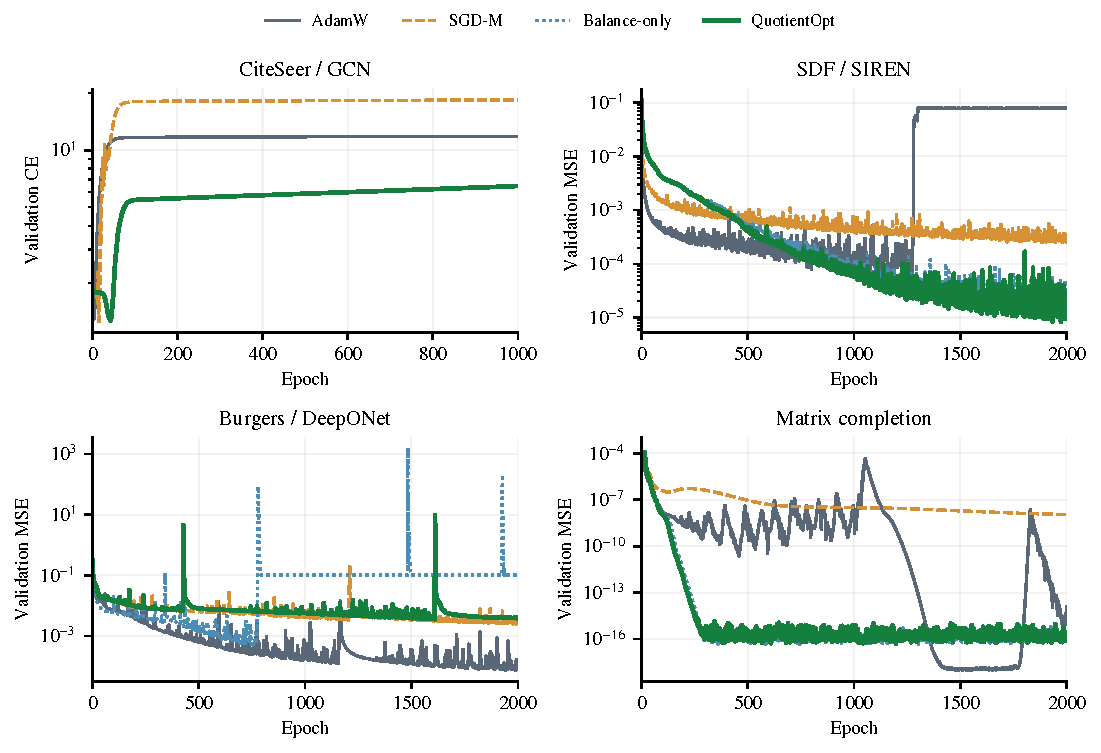
\includegraphics[width=.99\linewidth]{figures/new_task_complete_curves.pdf}
\captionof{figure}{All completed new-task comparison blocks, including unfavorable outcomes. For each method, validation loss selects the learning rate and checkpoint under the fixed rule; the entire selected run is plotted, with no smoothing or interval truncation. The curves are validation measurements, not IID risk certificates.}
\label{fig:new-task-curves}

\end{minipage}\par\medskip

\FloatBarrier
\paragraph{Descriptive validation iteration profiles.}
For regression tasks we additionally report the complete family of
relative-MSE targets $\{10^{-1},10^{-2},10^{-3},10^{-4},10^{-6}\}$.
With the same initial model and validation data for all methods,
define the finite-prefix tuning envelope
\begin{equation}
 e_{m,t}=\min_{\lambda\in\Lambda_m}
 \min_{0\le s\le\min\{t,T_{m,\lambda}\}}
 \frac{L_{\rm val}(z_{m,\lambda,s})}{L_{\rm val}(z_0)},
 \qquad
 \tau_m(a)=\inf\{t:e_{m,t}\le a\}.
\end{equation}
Every method has the same 13 optimizer settings. Retained finite
prefixes of stopped runs are eligible, so failed configurations do not
erase a baseline's earlier finite progress. An unreached target is
censored at the horizon. These are descriptive validation tuning
profiles, with test metrics excluded, rather than an independently
registered confirmation or a single executable optimizer trajectory.
They compare iteration budgets; shared-machine wall times are not a
controlled speed benchmark. The common initial validation scale is
checked against saved initial model states across methods and settings.
\par\medskip\noindent\begin{minipage}{\linewidth}

\centering\small
\captionof{table}{All descriptive validation-MSE targets in the new regression tasks. Each entry is the first epoch at which the validation tuning profile reaches the stated fraction of the common initial validation MSE. Every method has 13 optimizer settings; finite prefixes of later-stopped runs are eligible. A dash denotes an unreached target by epoch 2000. These are validation-selected iteration profiles, not wall-clock benchmarks or single executable training trajectories.}
\label{tab:new-task-hitting}
\begin{tabular}{lrrrrr}
\toprule Task & Relative target & AdamW & SGD-M & Balance & QO\\\midrule
SDF / SIREN & $10^{-1}$ & 2 & 2 & 2 & 2\\
SDF / SIREN & $10^{-2}$ & 11 & 28 & 16 & 17\\
SDF / SIREN & $10^{-3}$ & 157 & 1350 & 403 & 403\\
SDF / SIREN & $10^{-4}$ & \textemdash & \textemdash & 1183 & 1142\\
SDF / SIREN & $10^{-6}$ & \textemdash & \textemdash & \textemdash & \textemdash\\
Burgers / DeepONet & $10^{-1}$ & 73 & 292 & 47 & 47\\
Burgers / DeepONet & $10^{-2}$ & 297 & \textemdash & 651 & 584\\
Burgers / DeepONet & $10^{-3}$ & \textemdash & \textemdash & \textemdash & \textemdash\\
Burgers / DeepONet & $10^{-4}$ & \textemdash & \textemdash & \textemdash & \textemdash\\
Burgers / DeepONet & $10^{-6}$ & \textemdash & \textemdash & \textemdash & \textemdash\\
Matrix completion & $10^{-1}$ & 16 & 25 & 19 & 19\\
Matrix completion & $10^{-2}$ & 43 & 57 & 48 & 45\\
Matrix completion & $10^{-3}$ & 67 & 502 & 71 & 69\\
Matrix completion & $10^{-4}$ & 138 & \textemdash & 117 & 107\\
Matrix completion & $10^{-6}$ & 215 & \textemdash & 162 & 150\\
\bottomrule
\end{tabular}

\end{minipage}\par\medskip
\par\medskip\noindent\begin{minipage}{\linewidth}

\centering
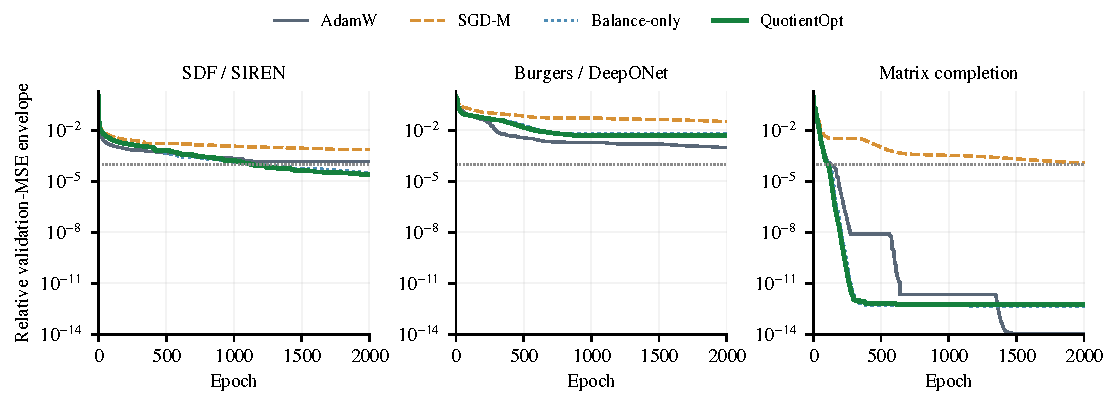
\includegraphics[width=.99\linewidth]{figures/new_task_convergence_profiles.pdf}
\captionof{figure}{Validation tuning envelopes from every completed regression-task block. At each epoch the envelope takes the best finite validation checkpoint among all 13 settings and earlier epochs, including prefixes of later-stopped trials. It is a descriptive equal-budget tuning profile, not one optimizer trajectory. The horizontal line is the $10^{-4}$ relative-MSE target; Table~\ref{tab:new-task-hitting} retains all five targets. Values below $10^{-14}$ are drawn at the plotting floor for legibility.}
\label{fig:new-task-convergence}

\end{minipage}\par\medskip

\FloatBarrier
\begingroup\small\setlength{\tabcolsep}{3pt}
\begin{longtable}{p{.34\linewidth}p{.09\linewidth}rrrr}
\caption{All attempted configurations in the new four-family expansion at this snapshot. Entries are validation-selected test losses, not test-minimized checkpoints; LR is the factor learning rate. Non-factor LR equals LR for the original nine settings through 0.1 and is fixed at $10^{-3}$ for the four added factor LRs 0.3, 1, 3, and 10. E is the selected epoch. C denotes a completed full-horizon run; F denotes a stopped run, whose best finite validation checkpoint is reported when available. Pending and running attempts have no final result and are omitted from this table. Their counts remain in Table~\ref{tab:new-task-status}.}\label{tab:new-task-all}\\
\toprule Task / method & LR & E & Val.\ score & Test loss & Status\\\midrule\endfirsthead
\toprule Task / method & LR & E & Val.\ score & Test loss & Status\\\midrule\endhead
CiteSeer / GCN / AdamW & 1e-05 & 1000 & 1.7272 & 1.7143 & C\\
CiteSeer / GCN / SGD-M & 1e-05 & 1000 & 1.7757 & 1.7693 & C\\
CiteSeer / GCN / Balance-only & 1e-05 & 1000 & 1.7757 & 1.7692 & C\\
\rowcolor{oursbg}CiteSeer / GCN / QuotientOpt & 1e-05 & 1000 & 1.7757 & 1.7692 & C\\
SDF / SIREN / AdamW & 1e-05 & 2000 & 0.0012 & 0.0015 & C\\
SDF / SIREN / SGD-M & 1e-05 & 2000 & 0.0049 & 0.0050 & C\\
SDF / SIREN / Balance-only & 1e-05 & 2000 & 0.0072 & 0.0063 & C\\
\rowcolor{oursbg}SDF / SIREN / QuotientOpt & 1e-05 & 2000 & 0.0072 & 0.0063 & C\\
Burgers / DeepONet / AdamW & 1e-05 & 2000 & 0.0014 & 0.0016 & C\\
Burgers / DeepONet / SGD-M & 1e-05 & 2000 & 0.0096 & 0.0113 & C\\
Burgers / DeepONet / Balance-only & 1e-05 & 2000 & 0.0096 & 0.0113 & C\\
\rowcolor{oursbg}Burgers / DeepONet / QuotientOpt & 1e-05 & 2000 & 0.0096 & 0.0113 & C\\
Matrix completion / AdamW & 1e-05 & 2000 & $7.56\!\times\!10^{-5}$ & $7.48\!\times\!10^{-5}$ & C\\
Matrix completion / SGD-M & 1e-05 & 725 & $9.10\!\times\!10^{-5}$ & $9.08\!\times\!10^{-5}$ & C\\
Matrix completion / Balance-only & 1e-05 & 2000 & $9.11\!\times\!10^{-5}$ & $9.11\!\times\!10^{-5}$ & C\\
\rowcolor{oursbg}Matrix completion / QuotientOpt & 1e-05 & 2000 & $9.11\!\times\!10^{-5}$ & $9.11\!\times\!10^{-5}$ & C\\
CiteSeer / GCN / AdamW & 3e-05 & 695 & 1.4035 & 1.3374 & C\\
CiteSeer / GCN / SGD-M & 3e-05 & 1000 & 1.3855 & 1.2792 & C\\
CiteSeer / GCN / Balance-only & 3e-05 & 1000 & 1.3852 & 1.2795 & C\\
\rowcolor{oursbg}CiteSeer / GCN / QuotientOpt & 3e-05 & 1000 & 1.3852 & 1.2795 & C\\
SDF / SIREN / AdamW & 3e-05 & 2000 & $3.56\!\times\!10^{-4}$ & $3.74\!\times\!10^{-4}$ & C\\
SDF / SIREN / SGD-M & 3e-05 & 1991 & 0.0020 & 0.0021 & C\\
SDF / SIREN / Balance-only & 3e-05 & 2000 & 0.0034 & 0.0031 & C\\
\rowcolor{oursbg}SDF / SIREN / QuotientOpt & 3e-05 & 2000 & 0.0033 & 0.0031 & C\\
Burgers / DeepONet / AdamW & 3e-05 & 2000 & $5.20\!\times\!10^{-4}$ & $5.85\!\times\!10^{-4}$ & C\\
Burgers / DeepONet / SGD-M & 3e-05 & 2000 & 0.0081 & 0.0095 & C\\
Burgers / DeepONet / Balance-only & 3e-05 & 2000 & 0.0082 & 0.0096 & C\\
\rowcolor{oursbg}Burgers / DeepONet / QuotientOpt & 3e-05 & 2000 & 0.0081 & 0.0096 & C\\
Matrix completion / AdamW & 3e-05 & 2000 & $2.08\!\times\!10^{-5}$ & $2.20\!\times\!10^{-5}$ & C\\
Matrix completion / SGD-M & 3e-05 & 247 & $9.10\!\times\!10^{-5}$ & $9.08\!\times\!10^{-5}$ & C\\
Matrix completion / Balance-only & 3e-05 & 2000 & $9.10\!\times\!10^{-5}$ & $9.10\!\times\!10^{-5}$ & C\\
\rowcolor{oursbg}Matrix completion / QuotientOpt & 3e-05 & 2000 & $9.10\!\times\!10^{-5}$ & $9.10\!\times\!10^{-5}$ & C\\
CiteSeer / GCN / AdamW & 0.0001 & 231 & 1.3392 & 1.2774 & C\\
CiteSeer / GCN / SGD-M & 0.0001 & 355 & 1.3561 & 1.2243 & C\\
CiteSeer / GCN / Balance-only & 0.0001 & 356 & 1.3555 & 1.2241 & C\\
\rowcolor{oursbg}CiteSeer / GCN / QuotientOpt & 0.0001 & 356 & 1.3560 & 1.2244 & C\\
SDF / SIREN / AdamW & 0.0001 & 1989 & $1.62\!\times\!10^{-4}$ & $1.64\!\times\!10^{-4}$ & C\\
SDF / SIREN / SGD-M & 0.0001 & 1998 & 0.0011 & 0.0011 & C\\
SDF / SIREN / Balance-only & 0.0001 & 2000 & $8.87\!\times\!10^{-4}$ & $8.74\!\times\!10^{-4}$ & C\\
\rowcolor{oursbg}SDF / SIREN / QuotientOpt & 0.0001 & 2000 & $6.94\!\times\!10^{-4}$ & $7.05\!\times\!10^{-4}$ & C\\
Burgers / DeepONet / AdamW & 0.0001 & 1990 & $1.34\!\times\!10^{-4}$ & $1.66\!\times\!10^{-4}$ & C\\
Burgers / DeepONet / SGD-M & 0.0001 & 1988 & 0.0063 & 0.0074 & C\\
Burgers / DeepONet / Balance-only & 0.0001 & 1995 & 0.0064 & 0.0076 & C\\
\rowcolor{oursbg}Burgers / DeepONet / QuotientOpt & 0.0001 & 1983 & 0.0064 & 0.0076 & C\\
Matrix completion / AdamW & 0.0001 & 2000 & $1.75\!\times\!10^{-6}$ & $1.77\!\times\!10^{-6}$ & C\\
Matrix completion / SGD-M & 0.0001 & 80 & $9.10\!\times\!10^{-5}$ & $9.08\!\times\!10^{-5}$ & C\\
Matrix completion / Balance-only & 0.0001 & 2000 & $9.08\!\times\!10^{-5}$ & $9.06\!\times\!10^{-5}$ & C\\
\rowcolor{oursbg}Matrix completion / QuotientOpt & 0.0001 & 2000 & $9.08\!\times\!10^{-5}$ & $9.06\!\times\!10^{-5}$ & C\\
CiteSeer / GCN / AdamW & 0.0003 & 96 & 1.3091 & 1.2485 & C\\
CiteSeer / GCN / SGD-M & 0.0003 & 139 & 1.3492 & 1.2123 & C\\
CiteSeer / GCN / Balance-only & 0.0003 & 139 & 1.3489 & 1.2128 & C\\
\rowcolor{oursbg}CiteSeer / GCN / QuotientOpt & 0.0003 & 138 & 1.3492 & 1.2152 & C\\
SDF / SIREN / AdamW & 0.0003 & 1994 & $1.22\!\times\!10^{-4}$ & $1.21\!\times\!10^{-4}$ & C\\
SDF / SIREN / SGD-M & 0.0003 & 1994 & $6.41\!\times\!10^{-4}$ & $6.72\!\times\!10^{-4}$ & C\\
SDF / SIREN / Balance-only & 0.0003 & 1997 & $6.74\!\times\!10^{-5}$ & $6.49\!\times\!10^{-5}$ & C\\
\rowcolor{oursbg}SDF / SIREN / QuotientOpt & 0.0003 & 1998 & $7.49\!\times\!10^{-5}$ & $8.96\!\times\!10^{-5}$ & C\\
Burgers / DeepONet / AdamW & 0.0003 & 1941 & $7.40\!\times\!10^{-5}$ & $8.66\!\times\!10^{-5}$ & C\\
Burgers / DeepONet / SGD-M & 0.0003 & 1977 & 0.0045 & 0.0053 & C\\
Burgers / DeepONet / Balance-only & 0.0003 & 1978 & 0.0047 & 0.0056 & C\\
\rowcolor{oursbg}Burgers / DeepONet / QuotientOpt & 0.0003 & 1997 & 0.0046 & 0.0055 & C\\
Matrix completion / AdamW & 0.0003 & 2000 & $3.14\!\times\!10^{-7}$ & $2.71\!\times\!10^{-7}$ & C\\
Matrix completion / SGD-M & 0.0003 & 2000 & $3.99\!\times\!10^{-5}$ & $3.87\!\times\!10^{-5}$ & C\\
Matrix completion / Balance-only & 0.0003 & 2000 & $9.02\!\times\!10^{-5}$ & $8.97\!\times\!10^{-5}$ & C\\
\rowcolor{oursbg}Matrix completion / QuotientOpt & 0.0003 & 2000 & $9.02\!\times\!10^{-5}$ & $8.97\!\times\!10^{-5}$ & C\\
CiteSeer / GCN / AdamW & 0.001 & 38 & 1.3143 & 1.2552 & C\\
CiteSeer / GCN / SGD-M & 0.001 & 53 & 1.3352 & 1.2125 & C\\
CiteSeer / GCN / Balance-only & 0.001 & 53 & 1.3358 & 1.2128 & C\\
\rowcolor{oursbg}CiteSeer / GCN / QuotientOpt & 0.001 & 53 & 1.3357 & 1.2127 & C\\
SDF / SIREN / AdamW & 0.001 & 1964 & $5.65\!\times\!10^{-5}$ & $8.43\!\times\!10^{-5}$ & C\\
SDF / SIREN / SGD-M & 0.001 & 1991 & $3.49\!\times\!10^{-4}$ & $3.97\!\times\!10^{-4}$ & C\\
SDF / SIREN / Balance-only & 0.001 & 1929 & $1.07\!\times\!10^{-5}$ & $1.10\!\times\!10^{-5}$ & C\\
\rowcolor{oursbg}SDF / SIREN / QuotientOpt & 0.001 & 1972 & $8.39\!\times\!10^{-6}$ & $9.36\!\times\!10^{-6}$ & C\\
Burgers / DeepONet / AdamW & 0.001 & 1957 & $1.45\!\times\!10^{-4}$ & $1.82\!\times\!10^{-4}$ & C\\
Burgers / DeepONet / SGD-M & 0.001 & 1977 & 0.0025 & 0.0030 & C\\
Burgers / DeepONet / Balance-only & 0.001 & 1944 & 0.0030 & 0.0036 & C\\
\rowcolor{oursbg}Burgers / DeepONet / QuotientOpt & 0.001 & 1608 & 0.0036 & 0.0042 & C\\
Matrix completion / AdamW & 0.001 & 2000 & $6.64\!\times\!10^{-8}$ & $7.12\!\times\!10^{-8}$ & C\\
Matrix completion / SGD-M & 0.001 & 2000 & $5.07\!\times\!10^{-6}$ & $4.95\!\times\!10^{-6}$ & C\\
Matrix completion / Balance-only & 0.001 & 2000 & $8.26\!\times\!10^{-5}$ & $8.12\!\times\!10^{-5}$ & C\\
\rowcolor{oursbg}Matrix completion / QuotientOpt & 0.001 & 2000 & $8.26\!\times\!10^{-5}$ & $8.12\!\times\!10^{-5}$ & C\\
CiteSeer / GCN / AdamW & 0.003 & 16 & 1.3068 & 1.2660 & C\\
CiteSeer / GCN / SGD-M & 0.003 & 28 & 1.3386 & 1.1922 & C\\
CiteSeer / GCN / Balance-only & 0.003 & 28 & 1.3401 & 1.1937 & C\\
\rowcolor{oursbg}CiteSeer / GCN / QuotientOpt & 0.003 & 28 & 1.3401 & 1.1937 & C\\
SDF / SIREN / AdamW & 0.003 & 1130 & $4.90\!\times\!10^{-5}$ & $6.03\!\times\!10^{-5}$ & C\\
SDF / SIREN / SGD-M & 0.003 & 1947 & $2.47\!\times\!10^{-4}$ & $2.42\!\times\!10^{-4}$ & C\\
SDF / SIREN / Balance-only & 0.003 & 1993 & $2.32\!\times\!10^{-5}$ & $2.63\!\times\!10^{-5}$ & C\\
\rowcolor{oursbg}SDF / SIREN / QuotientOpt & 0.003 & 1943 & $2.30\!\times\!10^{-5}$ & $2.40\!\times\!10^{-5}$ & C\\
Burgers / DeepONet / AdamW & 0.003 & 535 & $2.93\!\times\!10^{-4}$ & $3.50\!\times\!10^{-4}$ & C\\
Burgers / DeepONet / SGD-M & 0.003 & 585 & 0.0041 & 0.0049 & C\\
Burgers / DeepONet / Balance-only & 0.003 & 1978 & 0.0029 & 0.0035 & C\\
\rowcolor{oursbg}Burgers / DeepONet / QuotientOpt & 0.003 & 1519 & 0.0040 & 0.0047 & C\\
Matrix completion / AdamW & 0.003 & 1999 & $2.11\!\times\!10^{-8}$ & $2.20\!\times\!10^{-8}$ & C\\
Matrix completion / SGD-M & 0.003 & 2000 & $2.01\!\times\!10^{-6}$ & $1.84\!\times\!10^{-6}$ & C\\
Matrix completion / Balance-only & 0.003 & 2000 & $1.35\!\times\!10^{-5}$ & $1.26\!\times\!10^{-5}$ & C\\
\rowcolor{oursbg}Matrix completion / QuotientOpt & 0.003 & 2000 & $1.35\!\times\!10^{-5}$ & $1.26\!\times\!10^{-5}$ & C\\
CiteSeer / GCN / AdamW & 0.01 & 7 & 1.3692 & 1.3316 & C\\
CiteSeer / GCN / SGD-M & 0.01 & 19 & 1.3442 & 1.2166 & C\\
CiteSeer / GCN / Balance-only & 0.01 & 19 & 1.3505 & 1.2240 & C\\
\rowcolor{oursbg}CiteSeer / GCN / QuotientOpt & 0.01 & 19 & 1.3501 & 1.2234 & C\\
SDF / SIREN / AdamW & 0.01 & 39 & 0.0780 & 0.0747 & C\\
SDF / SIREN / SGD-M & 0.01 & 651 & $5.43\!\times\!10^{-4}$ & $5.49\!\times\!10^{-4}$ & C\\
SDF / SIREN / Balance-only & 0.01 & 412 & $2.46\!\times\!10^{-4}$ & $2.54\!\times\!10^{-4}$ & C\\
\rowcolor{oursbg}SDF / SIREN / QuotientOpt & 0.01 & 485 & $2.10\!\times\!10^{-4}$ & $2.13\!\times\!10^{-4}$ & C\\
Burgers / DeepONet / AdamW & 0.01 & 417 & 0.0040 & 0.0046 & C\\
Burgers / DeepONet / SGD-M & 0.01 & 41 & 0.1007 & 0.1177 & C\\
Burgers / DeepONet / Balance-only & 0.01 & 570 & 0.0069 & 0.0081 & C\\
\rowcolor{oursbg}Burgers / DeepONet / QuotientOpt & 0.01 & 770 & 0.0055 & 0.0065 & F\\
Matrix completion / AdamW & 0.01 & 2000 & $3.70\!\times\!10^{-10}$ & $3.87\!\times\!10^{-10}$ & C\\
Matrix completion / SGD-M & 0.01 & 2000 & $5.99\!\times\!10^{-7}$ & $5.46\!\times\!10^{-7}$ & C\\
Matrix completion / Balance-only & 0.01 & 2000 & $2.20\!\times\!10^{-6}$ & $2.15\!\times\!10^{-6}$ & C\\
\rowcolor{oursbg}Matrix completion / QuotientOpt & 0.01 & 2000 & $2.20\!\times\!10^{-6}$ & $2.15\!\times\!10^{-6}$ & C\\
CiteSeer / GCN / AdamW & 0.03 & 5 & 1.5255 & 1.5701 & C\\
CiteSeer / GCN / SGD-M & 0.03 & 27 & 1.3885 & 1.3170 & C\\
CiteSeer / GCN / Balance-only & 0.03 & 26 & 1.5585 & 1.4382 & C\\
\rowcolor{oursbg}CiteSeer / GCN / QuotientOpt & 0.03 & 26 & 1.5585 & 1.4382 & C\\
SDF / SIREN / AdamW & 0.03 & 9 & 0.0797 & 0.0746 & C\\
SDF / SIREN / SGD-M & 0.03 & 6 & 0.0786 & 0.0727 & F\\
SDF / SIREN / Balance-only & 0.03 & 147 & 0.0015 & 0.0016 & C\\
\rowcolor{oursbg}SDF / SIREN / QuotientOpt & 0.03 & 145 & 0.0020 & 0.0020 & C\\
Burgers / DeepONet / AdamW & 0.03 & 1278 & 0.0260 & 0.0242 & C\\
Burgers / DeepONet / SGD-M & 0.03 & 41 & 0.1007 & 0.1177 & C\\
Burgers / DeepONet / Balance-only & 0.03 & 62 & 0.1007 & 0.1177 & C\\
\rowcolor{oursbg}Burgers / DeepONet / QuotientOpt & 0.03 & 39 & 0.1007 & 0.1177 & F\\
Matrix completion / AdamW & 0.03 & 1540 & $9.61\!\times\!10^{-19}$ & $1.06\!\times\!10^{-18}$ & C\\
Matrix completion / SGD-M & 0.03 & 2000 & $2.06\!\times\!10^{-7}$ & $1.94\!\times\!10^{-7}$ & C\\
Matrix completion / Balance-only & 0.03 & 2000 & $3.64\!\times\!10^{-7}$ & $3.23\!\times\!10^{-7}$ & C\\
\rowcolor{oursbg}Matrix completion / QuotientOpt & 0.03 & 2000 & $3.63\!\times\!10^{-7}$ & $3.23\!\times\!10^{-7}$ & C\\
CiteSeer / GCN / AdamW & 0.1 & 22 & 1.6835 & 1.7497 & C\\
CiteSeer / GCN / SGD-M & 0.1 & 81 & 1.7301 & 1.7913 & C\\
CiteSeer / GCN / Balance-only & 0.1 & 100 & 1.7300 & 1.8034 & C\\
\rowcolor{oursbg}CiteSeer / GCN / QuotientOpt & 0.1 & 113 & 1.7375 & 1.8088 & C\\
SDF / SIREN / AdamW & 0.1 & 5 & 0.0900 & 0.0853 & C\\
SDF / SIREN / SGD-M & 0.1 & 1 & 0.3478 & 0.3722 & F\\
SDF / SIREN / Balance-only & 0.1 & 11 & 0.0791 & 0.0742 & F\\
\rowcolor{oursbg}SDF / SIREN / QuotientOpt & 0.1 & 13 & 0.0797 & 0.0755 & F\\
Burgers / DeepONet / AdamW & 0.1 & 1726 & 0.1006 & 0.1176 & C\\
Burgers / DeepONet / SGD-M & 0.1 & 170 & 0.0524 & 0.0578 & C\\
Burgers / DeepONet / Balance-only & 0.1 & 36 & 0.1007 & 0.1177 & C\\
\rowcolor{oursbg}Burgers / DeepONet / QuotientOpt & 0.1 & -- & \textemdash & \textemdash & F\\
Matrix completion / AdamW & 0.1 & 641 & $1.96\!\times\!10^{-16}$ & $1.88\!\times\!10^{-16}$ & C\\
Matrix completion / SGD-M & 0.1 & 2000 & $5.11\!\times\!10^{-8}$ & $5.25\!\times\!10^{-8}$ & C\\
Matrix completion / Balance-only & 0.1 & 2000 & $4.59\!\times\!10^{-8}$ & $3.90\!\times\!10^{-8}$ & C\\
\rowcolor{oursbg}Matrix completion / QuotientOpt & 0.1 & 2000 & $4.57\!\times\!10^{-8}$ & $3.89\!\times\!10^{-8}$ & C\\
CiteSeer / GCN / AdamW & 0.3 & 4 & 1.2942 & 1.3762 & C\\
CiteSeer / GCN / SGD-M & 0.3 & 33 & 1.3254 & 1.2699 & C\\
CiteSeer / GCN / Balance-only & 0.3 & 48 & 1.2749 & 1.1835 & C\\
\rowcolor{oursbg}CiteSeer / GCN / QuotientOpt & 0.3 & 48 & 1.2756 & 1.1842 & C\\
SDF / SIREN / AdamW & 0.3 & 182 & 0.0774 & 0.0726 & C\\
SDF / SIREN / SGD-M & 0.3 & 1 & 0.2931 & 0.3260 & F\\
SDF / SIREN / Balance-only & 0.3 & 1994 & $1.50\!\times\!10^{-4}$ & $1.70\!\times\!10^{-4}$ & C\\
\rowcolor{oursbg}SDF / SIREN / QuotientOpt & 0.3 & 1954 & $1.37\!\times\!10^{-4}$ & $1.54\!\times\!10^{-4}$ & C\\
Burgers / DeepONet / AdamW & 0.3 & 61 & 0.0317 & 0.0314 & C\\
Burgers / DeepONet / SGD-M & 0.3 & 22 & 0.1007 & 0.1177 & C\\
Burgers / DeepONet / Balance-only & 0.3 & 762 & $4.93\!\times\!10^{-4}$ & $5.85\!\times\!10^{-4}$ & C\\
\rowcolor{oursbg}Burgers / DeepONet / QuotientOpt & 0.3 & 910 & $3.62\!\times\!10^{-4}$ & $4.37\!\times\!10^{-4}$ & F\\
Matrix completion / AdamW & 0.3 & 2000 & $3.13\!\times\!10^{-9}$ & $2.98\!\times\!10^{-9}$ & C\\
Matrix completion / SGD-M & 0.3 & 2000 & $1.10\!\times\!10^{-8}$ & $1.17\!\times\!10^{-8}$ & C\\
Matrix completion / Balance-only & 0.3 & 2000 & $4.87\!\times\!10^{-9}$ & $4.25\!\times\!10^{-9}$ & C\\
\rowcolor{oursbg}Matrix completion / QuotientOpt & 0.3 & 2000 & $4.67\!\times\!10^{-9}$ & $4.08\!\times\!10^{-9}$ & C\\
CiteSeer / GCN / AdamW & 1 & 4 & 2.9122 & 2.9363 & C\\
CiteSeer / GCN / SGD-M & 1 & 26 & 1.3674 & 1.3193 & C\\
CiteSeer / GCN / Balance-only & 1 & 43 & 1.2690 & 1.2168 & C\\
\rowcolor{oursbg}CiteSeer / GCN / QuotientOpt & 1 & 43 & 1.2671 & 1.2163 & C\\
SDF / SIREN / AdamW & 1 & 67 & 0.0774 & 0.0727 & C\\
SDF / SIREN / SGD-M & 1 & -- & \textemdash & \textemdash & F\\
SDF / SIREN / Balance-only & 1 & 1980 & $1.36\!\times\!10^{-4}$ & $1.32\!\times\!10^{-4}$ & C\\
\rowcolor{oursbg}SDF / SIREN / QuotientOpt & 1 & 1995 & $1.40\!\times\!10^{-4}$ & $1.73\!\times\!10^{-4}$ & C\\
Burgers / DeepONet / AdamW & 1 & 36 & 0.1007 & 0.1177 & C\\
Burgers / DeepONet / SGD-M & 1 & 300 & 0.1007 & 0.1177 & C\\
Burgers / DeepONet / Balance-only & 1 & 29 & 0.1007 & 0.1177 & C\\
\rowcolor{oursbg}Burgers / DeepONet / QuotientOpt & 1 & 1 & 0.1332 & 0.1559 & F\\
Matrix completion / AdamW & 1 & 2000 & $5.79\!\times\!10^{-7}$ & $5.05\!\times\!10^{-7}$ & C\\
Matrix completion / SGD-M & 1 & 6 & $2.67\!\times\!10^{-5}$ & $2.70\!\times\!10^{-5}$ & F\\
Matrix completion / Balance-only & 1 & 2000 & $4.69\!\times\!10^{-7}$ & $1.98\!\times\!10^{-7}$ & C\\
\rowcolor{oursbg}Matrix completion / QuotientOpt & 1 & 2000 & $3.97\!\times\!10^{-7}$ & $1.87\!\times\!10^{-7}$ & C\\
CiteSeer / GCN / AdamW & 3 & 6 & 12.0411 & 14.8568 & C\\
CiteSeer / GCN / SGD-M & 3 & 23 & 1.3106 & 1.4144 & C\\
CiteSeer / GCN / Balance-only & 3 & 32 & 1.3635 & 1.3001 & C\\
\rowcolor{oursbg}CiteSeer / GCN / QuotientOpt & 3 & 32 & 1.3628 & 1.2997 & C\\
SDF / SIREN / AdamW & 3 & 429 & 0.0775 & 0.0730 & C\\
SDF / SIREN / SGD-M & 3 & -- & \textemdash & \textemdash & F\\
SDF / SIREN / Balance-only & 3 & 1 & 0.3028 & 0.3246 & F\\
\rowcolor{oursbg}SDF / SIREN / QuotientOpt & 3 & 1 & 0.3035 & 0.3098 & F\\
Burgers / DeepONet / AdamW & 3 & 35 & 0.1007 & 0.1177 & C\\
Burgers / DeepONet / SGD-M & 3 & 549 & 0.1007 & 0.1177 & C\\
Burgers / DeepONet / Balance-only & 3 & 30 & 0.1007 & 0.1177 & C\\
\rowcolor{oursbg}Burgers / DeepONet / QuotientOpt & 3 & 1 & 77.1926 & 76.3920 & F\\
Matrix completion / AdamW & 3 & 2000 & $6.52\!\times\!10^{-6}$ & $6.32\!\times\!10^{-6}$ & C\\
Matrix completion / SGD-M & 3 & 2 & $1.41\!\times\!10^{-4}$ & $1.36\!\times\!10^{-4}$ & F\\
Matrix completion / Balance-only & 3 & 2000 & $1.69\!\times\!10^{-6}$ & $1.39\!\times\!10^{-6}$ & C\\
\rowcolor{oursbg}Matrix completion / QuotientOpt & 3 & 2000 & $1.21\!\times\!10^{-6}$ & $1.04\!\times\!10^{-6}$ & C\\
CiteSeer / GCN / AdamW & 10 & 7 & 147.0064 & 185.7595 & C\\
CiteSeer / GCN / SGD-M & 10 & 16 & 1.2514 & 1.2508 & C\\
CiteSeer / GCN / Balance-only & 10 & 24 & 1.3988 & 1.3532 & C\\
\rowcolor{oursbg}CiteSeer / GCN / QuotientOpt & 10 & 24 & 1.3975 & 1.3524 & C\\
SDF / SIREN / AdamW & 10 & 1249 & 0.0774 & 0.0730 & C\\
SDF / SIREN / SGD-M & 10 & -- & \textemdash & \textemdash & F\\
SDF / SIREN / Balance-only & 10 & -- & \textemdash & \textemdash & F\\
\rowcolor{oursbg}SDF / SIREN / QuotientOpt & 10 & -- & \textemdash & \textemdash & F\\
Burgers / DeepONet / AdamW & 10 & 1583 & 0.1005 & 0.1175 & C\\
Burgers / DeepONet / SGD-M & 10 & 40 & 0.1007 & 0.1177 & C\\
Burgers / DeepONet / Balance-only & 10 & 37 & 0.1007 & 0.1177 & C\\
\rowcolor{oursbg}Burgers / DeepONet / QuotientOpt & 10 & 1 & 16.4258 & 16.4429 & F\\
Matrix completion / AdamW & 10 & 1941 & $9.48\!\times\!10^{-5}$ & $9.59\!\times\!10^{-5}$ & C\\
Matrix completion / SGD-M & 10 & 1 & 0.0011 & 0.0011 & F\\
Matrix completion / Balance-only & 10 & 1133 & $4.10\!\times\!10^{-17}$ & $4.14\!\times\!10^{-17}$ & C\\
\rowcolor{oursbg}Matrix completion / QuotientOpt & 10 & 1197 & $5.03\!\times\!10^{-17}$ & $4.65\!\times\!10^{-17}$ & C\\
\bottomrule
\end{longtable}
\endgroup
\paragraph{Stopped-checkpoint sensitivity: Burgers / DeepONet / QuotientOpt.} The minimum-validation-score checkpoint when stopped trials are eligible occurs at learning rate $0.3$ and epoch 910, with test loss $4.37\!\times\!10^{-4}$. The run status is failed. Its score is retained as a sensitivity control; it is not presented as a completed full-horizon run.

\FloatBarrier
